
\documentclass{svmult-ddm}

\usepackage{mathptmx}       % selects Times Roman as basic font
\usepackage{helvet}         % selects Helvetica as sans-serif font
\usepackage{courier}        % selects Courier as typewriter font
\usepackage{type1cm}        % activate if the above 3 fonts are
                            % not available on your system
\usepackage{graphicx}        % standard LaTeX graphics tool

                             % when including figure files

\usepackage[bottom]{footmisc}% places footnotes at page bottom

\usepackage{amssymb}
\usepackage{amsfonts}
\usepackage{amsbsy}
\usepackage{amscd}
\usepackage{amstext}
\usepackage{amsmath}
%\usepackage{dsfont}
\usepackage[english]{babel}
\usepackage{color}
\usepackage{graphics}
\usepackage{epsfig}
\usepackage{subfigure} 
\usepackage{wrapfig}
\usepackage{psfrag}
\usepackage{color}
\usepackage{url}
\usepackage{verbatim}
\usepackage{algorithm}
\usepackage{algorithmic}

%\usepackage{amsmath}

\begin{document}

\title*{Pipeline Schwarz Waveform Relaxation}
  \titlerunning{Pipeline Schwarz Waveform Relaxation}

\author{Scott High, Pranjal Vachaspati, James Stevens}

\maketitle


\section{Introduction}
\label{prop_sec:introduction}

Schwarz Waveform Relaxation (SWR), introduced in \cite{bjorhus1995},
is a domain decomposition based method for solving time dependent
PDEs.
In contrast to classical Schwarz iterations, where
the time-dependent PDE is discretized in time and domain-decomposition
is applied to the sequence of steady-state problems, SWR solves {\em
  time-dependent} sub-problems; this relaxes synchronization of the
sub-problems and provides a means to couple disparate solvers applied
to individual sub-problems,
Pipeline Schwarz waveform relaxation (PSWR), introduced in \cite{ongpipeline},
extends the spatial parallelism of SWR methods to the time domain by
computing successive iterations in a pipeline fashion.

\section{Problem Description}
\label{prop_sec:waveform}

Denote the PDE of interest as 
\begin{alignat}{2}
  \label{prop_eqn:pde1}
  u_t =&  \mathcal{L}(t,u), \quad &(x,t)\in \Omega\times[0,T]\\
  \nonumber
  u(x,0) =& f(x), \quad &x \in \Omega \\
  \nonumber
  u(z,t) =& g(z,t), \quad &z \in \partial\Omega. 
\end{alignat}
Consider a partitioning of the domain, $\Omega = \cup_i\Omega_i$.
The domains in the partition may be overlapping or non-overlapping.
Let $u_i$ denote the solution on sub-domain $\Omega_i$.
Then, equation~(\ref{prop_eqn:pde1}) can be decomposed into a
coupled system of equations,
\begin{alignat}{2}
  \label{prop_eqn:pde2}
  (u_i)_t =&  \mathcal{L}(t,u_i), &(x,t)\in \Omega_i\times[0,T]\\
  \nonumber
  u_i(x,0) =& f(x),  &x \in \Omega_i \\
  \nonumber
  u_i(z,t) =& g(z,t),  &z \in \partial\Omega_i\cap\partial\Omega, \\
  \nonumber
  \mathcal{T}_{ij}(u_{i}(z,t)) =& \mathcal{T}_{ij}(u_{j}(z,t)), &z \in \partial\Omega_i\cap\partial\Omega_j.
\end{alignat}
where $T$ are transmission operators appropriate to the
equation~(\ref{prop_eqn:pde1}).  SWR decouples the system of
PDEs in equation~(\ref{prop_eqn:pde2}).  Let $u_i^{[k]}$
denote the $k$-th waveform iterate on sub-domain $\Omega_i$. After
specifying an initial estimate for the sub-domain solution on the
interfaces, $u_i^{[0]}(z,t),
z\in\partial\Omega_i\setminus\partial\Omega$, the SWR algorithm
iteratively solves PDEs (\ref{prop_eqn:pde3}) for waveform
iterates $k=1,2,\ldots$ until convergence,
\begin{alignat}{2}
  \label{prop_eqn:pde3}
  (u_i^{[k]})_t &=  \mathcal{L}(t,u_i^{[k]}), \quad &(x,t)\in \Omega_i\times[0,T]\\
  \nonumber
  u_i^{[k]}(x,0) &= f(x), \quad &x \in \Omega_i \\
  \nonumber
  u_i^{[k]}(z,t) &= g(z,t), \quad &z \in \partial\Omega_i\cap\partial\Omega, \\
  \nonumber
  \mathcal{T}_{ij}(u_{i}^{[k]}(z,t)) &= \mathcal{T}_{ij}(u_{j}^{[k-1]}(z,t)), \quad &z \in \partial\Omega_i\cap\partial\Omega_j.
\end{alignat}


Using a similar approach described in
\cite{ChristliebMacdonaldOng2010,MR1340665}, the relaxation framework can be
rewritten so that after initial start-up costs, multiple waveform
iterations can be computed in a pipeline-parallel fashion. A graphical
example of the PSWR algorithm for two subdomains is shown in
Figure~\ref{prop_sec:pswr_fig}.
\begin{figure}
  \centering
  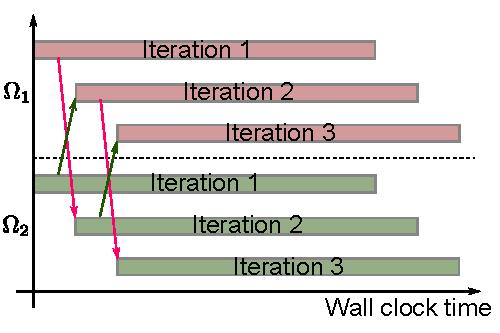
\includegraphics[width=0.5\textwidth]{figure1}
  \caption{The PSWR algorithm allows for multiple Schwarz waveform
    iterations to be simultaneously computed.  After an initial
    start-up cost, multiple iterates are computed in a pipeline
    fashion.}
  \label{prop_sec:pswr_fig}
\end{figure}

One of the key advantages of SWR methods is their flexibly. They can 
readily be made locally adaptive in time and space (within a domain),
and can even support different solvers in each domain. This makes them
ideal candidates for multiphysics applications and applications where
locally adaptive time stepping is needed, for example as discussed in
\cite{lemarie}

We intend to implement locally adaptive in time solutions to the 
2D anisotropic diffusion equation on a rectangular finite difference mesh.
To approximate real world multiphysics applications the diffusion constants
will be non-constant in the simulation domain.
To effectively amortize the overhead of having many processors idle
at the beginning and end of the simulation, we will solve for a
large number of time steps.
Backward time centered space (BTCS) stencils will be used to advance
the solution in time. A simple step doubling scheme will be used for local 
time adaptation.

We will use PETSc (Portable, Extensible Toolkit for Scientific Computation) to handle matrix creation and operations. PETSc is a toolkit for parallel scientific computing developed by Argonne National Laboratory \cite{InsertPETScCitationHere}. In particular, we will be making use of its tools for handling sparse matrices.

The pipelined algorithm has several features that make it an
attractive candidate for implementation in Charm++.  A PSWR iteration
can only proceed if boundary data (i.e. transmission conditions) from
the previous iterates are available; however, any iteration can
proceed for as long as it has updated boundary data regardless of the
current state of the next (or any other) iteration. In the original
MPI implementation, transmission data is exchanged after every time
step, resulting in lock step parallelism. The Charm framework's ability
to buffer messages and dynamically schedule processes can be used to
relax this tight synchronization, better exploiting the problem's
inherent parallelism. The use of overdecomposition will allow the 
Charm++ runtime to mitigate the load imbalance which results from 
adaptation in time.

\section{Parallel Implementation}
The basic structure of the parallel code is presented in Figure \ref{fig:sdag}. 
A given cell can start processing once it has received the boundary values from its neighbor with a smaller time index.
It then continues sending its result to its neighbors until it converges. The algorithm stops for a given cell if it converges or if all its neighbors converge.
 
\begin{figure}
\begin{verbatim}
  if (thisIndex.z > 0) {
    when(transmit(y, ind, isDone)) {
  	  updateBoundary(y);
    }
  }
  while(err < tol && nNeighbors > 0) {
    atomic {
      solve(x, y, thisIndex.z * timeSlice, (thisIndex.z + 1) * timeSlice, dt);
      for (i = 0; i < nNeighbors; i++) {
        neighbors[i].transmit(y, thisIndex, err < tol);
      }
      ++i;
    }
    for (i = 0; i < nNeighbors; i++) {
      when transmit(y, ind, isDone) atomic{
        updateBoundary(y);
        if (isDone) nNeighbors--;
      }
      
    if (thisIndex.z > 0)
      when updateTimestep(newdt) atomic {
      	dt = newdt;
      }
    else {
      dt = calcTimestep();
      thisArray[thisIndex.z + 1].updateTimestep(dt);
    }        
  }
\end{verbatim}
\label{fig:sdag}
\caption{The structure of the parallel algorithm.}
\end{figure}

%% BIBLIOGRAPHY %%%%%%%%%%%%%%%%%%%%%%%%%%%%%%%%%%%%%%%%%%%%%

\bibliographystyle{spmpsci}
\begin{thebibliography}{10}
\providecommand{\url}[1]{{#1}}
\providecommand{\urlprefix}{URL }
\expandafter\ifx\csname urlstyle\endcsname\relax
  \providecommand{\doi}[1]{DOI~\discretionary{}{}{}#1}\else
  \providecommand{\doi}{DOI~\discretionary{}{}{}\begingroup
  \urlstyle{rm}\Url}\fi

\bibitem{bjorhus1995}
Bj{\o}rhus, M.: On domain decomposition, subdomain iteration and waveform
  relaxation.
\newblock Ph.D. thesis, PhD thesis, University of Trondheim, Norway (1995)

\bibitem{ChristliebMacdonaldOng2010}
Christlieb, A., Macdonald, C., Ong, B.: Parallel high-order integrators.
\newblock SIAM J. Sci. Comput. \textbf{32}(2), 818--835 (2010)

\bibitem{MR1340665}
Vandewalle, S.G., Van~de Velde, E.F.: Space-time concurrent multigrid waveform
  relaxation.
\newblock Ann. Numer. Math. \textbf{1}(1-4), 347--360 (1994).
\newblock Scientific computation and differential equations (Auckland, 1993)

\bibitem{ongpipeline}
Ong, Benjamin and High, Scott and Kwok, Felix: Pipeline Schwarz Waveform Relaxation
\newblock Accepted

\bibitem{InsertPETScCitationHere}
InsertPETScCitationHere
\newblock InsertPETScCitationHere. InsertPETScCitationHere

\bibitem{lemarie}
Lemari{\'e}, F., Patrick, M., Debreu, L., Blayo, E.: {Sensitivity of an
  Ocean-Atmosphere Coupled Model to the Coupling Method : Study of Tropical
  Cyclone Erica}.
\newblock \urlprefix\url{http://hal.inria.fr/hal-00872496}


\end{thebibliography}


\end{document}				